\documentclass[12pt,a4paper]{article}
\usepackage[english]{babel}
\usepackage[utf8]{inputenc}
\usepackage{amssymb,amsmath}
\usepackage[all]{xy}
\usepackage{url}
\usepackage{graphicx}
\usepackage{color}
\newcommand{\angstrom}{\textup{\AA}}
\color{black}
\usepackage{geometry}
\usepackage[autostyle]{csquotes}
\usepackage{tikz}
\usetikzlibrary{bayesnet}
\def\UrlBreaks{\do\/\do-}
\usepackage{dcolumn}
\usepackage{booktabs}
\usepackage{tikz}
\usetikzlibrary{positioning,shapes,arrows}
\newcolumntype{M}[1]{D{.}{.}{1.#1}}
\usepackage{upquote} % Upright quotes for verbatim code
\usepackage{fancyvrb} % verbatim replacement that allows latex
\usepackage{float}
\usepackage{wrapfig}

\usepackage{amsmath}
\usepackage{algorithm}
\usepackage[noend]{algpseudocode}
\usepackage{listings}
\makeatletter
\def\BState{\State\hskip-\ALG@thistlm}
\makeatother
%Define the listing package
\usepackage{listings} %code highlighter
\usepackage{color} %use color
\definecolor{mygreen}{rgb}{0,0.6,0}
\definecolor{mygray}{rgb}{0.5,0.5,0.5}
\definecolor{mymauve}{rgb}{0.58,0,0.82}
 \usepackage{tikz} % Required for flow chart
\usetikzlibrary{shapes,arrows} % Tikz libraries required for the flow chart in the template

%Customize a bit the look
\lstset{ %
backgroundcolor=\color{white}, % choose the background color; you must add \usepackage{color} or \usepackage{xcolor}
basicstyle=\footnotesize, % the size of the fonts that are used for the code
breakatwhitespace=false, % sets if automatic breaks should only happen at whitespace
breaklines=true, % sets automatic line breaking
captionpos=b, % sets the caption-position to bottom
commentstyle=\color{mygreen}, % comment style
deletekeywords={...}, % if you want to delete keywords from the given language
escapeinside={\%*}{*)}, % if you want to add LaTeX within your code
extendedchars=true, % lets you use non-ASCII characters; for 8-bits encodings only, does not work with UTF-8
frame=single, % adds a frame around the code
keepspaces=true, % keeps spaces in text, useful for keeping indentation of code (possibly needs columns=flexible)
keywordstyle=\color{blue}, % keyword style
% language=Octave, % the language of the code
morekeywords={*,...}, % if you want to add more keywords to the set
numbers=left, % where to put the line-numbers; possible values are (none, left, right)
numbersep=5pt, % how far the line-numbers are from the code
numberstyle=\tiny\color{mygray}, % the style that is used for the line-numbers
rulecolor=\color{black}, % if not set, the frame-color may be changed on line-breaks within not-black text (e.g. comments (green here))
showspaces=false, % show spaces everywhere adding particular underscores; it overrides 'showstringspaces'
showstringspaces=false, % underline spaces within strings only
showtabs=false, % show tabs within strings adding particular underscores
stepnumber=1, % the step between two line-numbers. If it's 1, each line will be numbered
stringstyle=\color{mymauve}, % string literal style
tabsize=2, % sets default tabsize to 2 spaces
title=\lstname % show the filename of files included with \lstinputlisting; also try caption instead of title
}
%END of listing package%
 
\definecolor{darkgray}{rgb}{.4,.4,.4}
\definecolor{purple}{rgb}{0.65, 0.12, 0.82}
 
%define Javascript language
\lstdefinelanguage{JavaScript}{
keywords={typeof, new, true, false, catch, function, return, null, catch, switch, var, if, in, while, do, else, case, break},
keywordstyle=\color{blue}\bfseries,
ndkeywords={class, export, boolean, throw, implements, import, this},
ndkeywordstyle=\color{darkgray}\bfseries,
identifierstyle=\color{black},
sensitive=false,
comment=[l]{//},
morecomment=[s]{/*}{*/},
commentstyle=\color{purple}\ttfamily,
stringstyle=\color{red}\ttfamily,
morestring=[b]',
morestring=[b]"
}
 
\lstset{
language=JavaScript,
extendedchars=true,
basicstyle=\footnotesize\ttfamily,
showstringspaces=false,
showspaces=false,
numbers=left,
numberstyle=\footnotesize,
numbersep=9pt,
tabsize=2,
breaklines=true,
showtabs=false,
captionpos=b
}


\geometry{
	a4paper,
 	left=10mm,
 	right=10mm,
 	top=10mm,
 	bottom=10mm
}

\DefineVerbatimEnvironment{Highlighting}{Verbatim}{commandchars=\\\{\}}

\newcommand{\VerbatimStringTok}[1]{\textcolor[rgb]{0.25,0.44,0.63}{{#1}}}

\usepackage{hyperref}
\hypersetup{
    colorlinks,
    citecolor=black,
    filecolor=black,
    linkcolor=black,
    urlcolor=black
}


\begin{document}
\title{Interactive Graphics Homework 1}
\author{Michal Ostyk-Narbutt (1854051)\\ Prof. Marco Schaerf }

\maketitle


\begin{center}

\includegraphics[width=0.3\textwidth]{img/sapienza_logo.jpg}
\end{center}
\maketitle
%\tableofcontents

\section{Introduction}
This is a documentation report describing the techniques used in the First Homework for the Interactive Graphics course. Given a baseline file of a cube, the task was to modify it by
\begin{itemize}
\item  expanding the number of vertices (20-30) with each having a normal and texture coordinates.
\item adding a viewer position and a a perspective projection
\item computing the ModelView and Projection matrices in the Javascript application
\item adding two lights sources: Directional and a Spotlight
\item assigning to the object a material with the relevant properties
\item  Implementing a per-fragment shading model
\item adding a texture loaded from file, with the pixel color a combination of the color
computed using the lighting model and the texture.
\end{itemize}

\section{Documentation}
\subsection{Creating an irregular object}

\begin{wrapfigure}{r}{0.4\textwidth}
\centering
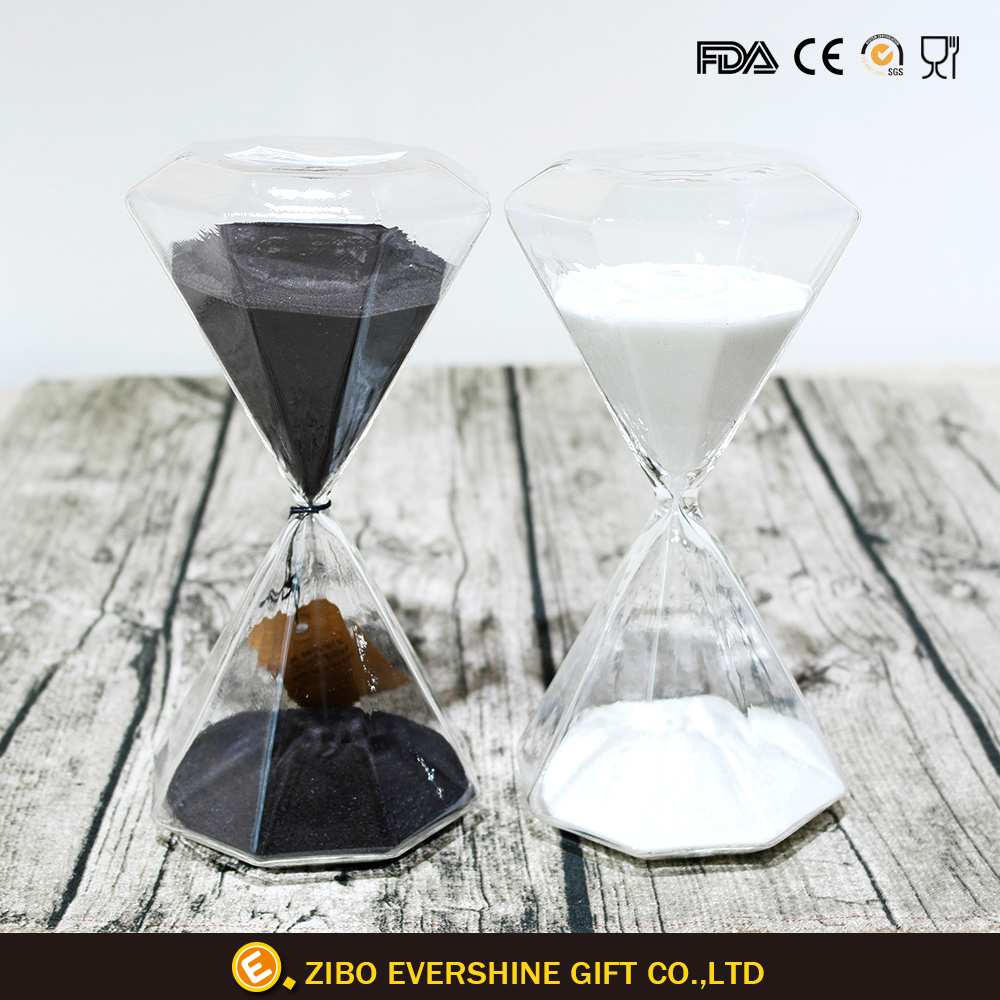
\includegraphics[width=0.3\textwidth, angle = 0]{img/hourglass.png}
\caption{Octagon Hourglass \cite{hourglass}}
\label{img:hourglass}
\end{wrapfigure}
My idea was to re-create an octagon Hourglass as seen in Figure \ref{img:hourglass}. In order to accomplish that task I decied to create out of a series of triangles (\texttt{tri function{}}) and quadrilaterals (\texttt{quad function{}}). However, unlike in Figure \ref{img:hourglass}, mine would have a more visible inner part.  



I modeled the vertices based 4 faces of different widths, with the top and bottom sharing one value for the width, and the inner "neck" of the hour composed of two octagons also sharing one value. To accomplish this task I decided to run the following python code which allowed me obtain various initial sizes. Moreover, the texture and normal coordinates were based on quadileteral and triangular properties respectively of each  (\texttt{tri function{}}) and (\texttt{quad function{}}) functions.
\clearpage
\begin{lstlisting}[caption={Getting values for the vertices},label={lst:python},language=python]
def getshapevalues(height_value, vertices=8, width=1):
    coords = []
    for ind, value  in enumerate(range(vertices), start=1):
        x = cos(2*value*pi/vertices) * width
        y = sin(2*value*pi/vertices) * width
        coords.append([x, y])
       return coords
\end{lstlisting}
The  code snippet in Listing \ref{lst:python} in Python is just a visual version of obtaining a polygon coordinates. These in reality would be checked for value and using strings formatted into JavaScript ready code. The result is show in Listing \ref{lst:bottomoctagon} below. 

\begin{lstlisting}[caption={Bottom Octagon example vertex defintions},label={lst:bottomoctagon},language=JavaScript]
vec4(0.6, 0.0, -1.0, 1.0), // point 0
vec4(0.3*Math.sqrt(2), 0.3*Math.sqrt(2), -1.0, 1.0), // point 1
vec4(0.0, 0.6, -1.0, 1.0), // point 2
vec4(-0.3*Math.sqrt(2), 0.3*Math.sqrt(2), -1.0, 1.0), // point 3
vec4(-0.6, 0.0, -1.0, 1.0), // point 4
vec4(-0.3*Math.sqrt(2), -0.3*Math.sqrt(2), -1.0, 1.0), // point 5
vec4(0.0, -0.6, -1.0, 1.0), // point 6
vec4(0.3*Math.sqrt(2), -0.3*Math.sqrt(2), -1.0, 1.0), // point 7
vec4(0, 0, -1.0, 1.0), // point (centroid) 8
\end{lstlisting}

Hence, using this procedure, from the four octagon faces, and inner points of the bottom and top face, a total of 34 vertices  (inner octagon centroids were not needed). The points were connected using.

\subsection{ModelView and Projection matrices}

Next, I added a viewer position, a projection and computed the ModelView and Projection matrices using a Javascript application. The ModelView was computed using the \texttt{lookAt} function which can concatenate with modeling transformations. Subsequently, sliders were added to the HTML file, which include the following transformations: radius, theta, phi, Near, Far, Scale, FOV (field of view), aspect. Additionaly for animation and asthetic reasons enabled buttons which through automatic increments of theta, and appropriate rotation matrices (\texttt{rz, ry, rx}) allow the rotation of the hourglass around the roll pitch yaw angles. Moreover, the shape can be translated along each of the X, Y, and Z world axes.

\subsection{Lighting: Directional and spotlight and Material}
The material and light are very much interconnected hence they will be described in one section together.
Both directional light and spotlight were required to be implemented with necessary elements depicted in Listing \ref{lst:lighting}. The directional light and spotlight were calculated appropriately  with these parameters as passing from each \texttt{gl.uniform4fv}  to the vertex shader. These were hence sent to the fragment shader via \texttt{N, L, E, L\_Directional, E\_Directional, L\_SpotLight, E\_SpotLight} parameters. There the material was blended with the shader model described in the next subsection, and multiplied by the spotlight outcome \texttt{spotfactor} which itself was based on the distance to the light source, and constant attenuation.

\begin{lstlisting}[caption={Light and Material parameters},label={lst:lighting},language=JavaScript]
var lightPosition, lightAmbient, lightDiffuse; // main light
var lightPositionDirectional, lightAmbientDirectional, lightAmbientDirectional;
var SpotlightAmbient, SpotlightDiffuse, SpotlightDirection;
var materialAmbient, materialDiffuse; //material
var constantAttenuation; // a single non changing  attenuation
var spotLightAngle, spotLightCutOff; // spotlight parameters
\end{lstlisting}

\subsection{Per-fragment shading model}
The per-fragment shading model used is called the Cartoon Shade Algorithm \cite{shade}
First, we had to calculate the illuminated diffuse color as in Equation \ref{eq1}, which is the vertex color. Next, the shadowed diffuse color in Equation \ref{eq2}. Finally once, we computed the value of the product of the unit vector from the light source to the vertex $\overrightarrow{L}$ and the unit vector
normal to the surface at the vertex  $\overrightarrow{n}$, we assign to the fragment the value based on the check in Equation 3. Note that the result of this product is the cosine of the angle between the two vectors. The resulting value would be either multiplied by the texture (described in the following seciton) or left as is a sum of $C_i$ and  $C_s$.
\begin{equation}\label{eq1}
C_i = a_g \times a_m + a_l \times a_m + d_l \times d_m  
\end{equation}
\begin{equation}\label{eq2}
C_s =  a_g \times a_m + a_l \times a_m
\end{equation}
\begin{equation}\label{eq3}
\text{ fragment assignment} =\begin{cases}
    C_i, & \text{if $\max(\overrightarrow{L} \cdot \overrightarrow{n}, 0)\geq0$}.\\
    C_s, & \text{if $\max(\overrightarrow{L} \cdot \overrightarrow{n}, 0)<0$}.
  \end{cases}
\end{equation}

\subsection{Texture from file}
The texture is simulated via png file from an online resource which depicts the the surface of the moon. The coordinates were pushed from predfined coordinates in both the  (\texttt{tri function{}}) and quadrilaterals (\texttt{quad function{}}) functions. Next, thanks to the \texttt{configureTexture} function there were mapped and sent to the fragment shader. The texture can be toggled on and off as requested.
\section{Conclusions}
\subsection{Advantages}
Please note that all CSS styling was taken from \cite{css}
\subsection{Disadvantages}


\begin{thebibliography}{1}

\bibitem{hourglass}   \url{http://evershinegift.com/Index.asp?Product420/742.html}
\bibitem{shade} Lake, Adam \& Marshall, Carl \& Harris, Mark \& Blackstein, Marc. (2000). Stylized Rendering Techniques For Scalable Real-Time 3D Animation. Proceedings of the Symposium on Non-Photorealistic Animation and Rendering. 10.1145/340916.340918.  \url{https://dl.acm.org/doi/pdf/10.1145/340916.340918}
\bibitem{docs} \url{https://www.khronos.org/registry/webgl/specs/latest/2.0}
\bibitem{css} \url{https://www.w3schools.com/css}

\end{thebibliography}
\end{document}
